Para empezar fácil, consideramos la forma más simple de un árbol de rangos.
Queremos responder consultas de suma de manera eficiente. La definición formal de nuestra tarea es: Tenemos una matriz $a[0 \dots n-1]$, y el árbol de segmentos debe poder encontrar la suma de elementos entre los índices $l$ y $r$ (es decir, calcular la suma $\sum_{i= l}^r a[i]$), y también manejar valores cambiantes de los elementos en la matriz (es decir, realizar asignaciones de la forma $a[i] = x$). El árbol de segmentos debería poder procesar ambas consultas en $O(\log n)$ tiempo.

Un árbol de rangos es una estructura de datos que permite responder consultas de rango sobre una matriz de manera efectiva, sin dejar de ser lo suficientemente flexible como para permitir la modificación de la matriz. Esto incluye encontrar la suma de los elementos consecutivos de la matriz $a[l…r]$, o encontrar el elemento mínimo en tal rango en el tiempo O($\log N$). Entre las respuestas a dichas consultas, el Árbol de segmentos permite modificar la matriz reemplazando un elemento, o incluso cambiar los elementos de un subsegmento completo (por ejemplo, asignando todos los elementos $a[l…r]$ a cualquier valor, o agregando un valor a todos los elementos en el subsegmento ).

\begin{figure}[h]
	\centering 
	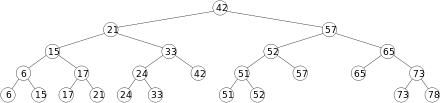
\includegraphics[scale=0.9]{img/range-tree}
	\caption{Representación de un árbol de rango}
	\label{contexto:figura1}
\end{figure}

\subsection{Operaciones}

\paragraph{Construción}
Un árbol de rangos se puede construir eficientemente de la siguiente manera:
Comenzamos en el nivel inferior, los vértices de las hojas.
Un vértice es un vértice de hoja, si su segmento correspondiente cubre un solo valor. Por lo tanto, simplemente podemos copiar los valores de los elementos $a[i]$. Sobre la base de estos valores, podemos calcular las sumas del nivel anterior. Y en base a ellos, podemos calcular las sumas de los anteriores, y repetir el procedimiento hasta llegar al vértice de la raíz. Es conveniente describir esta operación recursivamente:
comenzamos la construcción en el vértice raíz y el procedimiento de construcción, si se invoca en un vértice que no es hoja, primero construye recursivamente los dos vértices secundarios y luego suma las sumas calculadas de estos elementos secundarios. Si se llama en un vértice de hoja, simplemente usa el valor de la matriz.

La complejidad temporal de la construcción es $O(n)$.

\paragraph{Actualización}

Ahora queremos modificar un elemento específico en la matriz, digamos que queremos hacer la asignación $a[i] = x$.
Y tenemos que reconstruir el árbol de segmentos, de modo que corresponda a la nueva matriz modificada.

Esta consulta es más fácil que la consulta de suma. Cada nivel de un árbol de segmentos forma una partición de la matriz.
Por lo tanto, un elemento $a[i]$ solo contribuye a un segmento de cada nivel. Por lo tanto, solo se deben actualizar los vértices $O(\log n)$.

Es fácil ver que la solicitud de actualización se puede implementar mediante una función recursiva.
La función pasa el vértice del árbol actual, y recursivamente se llama a sí misma con uno de los dos vértices secundarios (el que contiene $a[i]$ en su segmento), y luego vuelve a calcular su valor de suma, similar a como se hace en el método de construcción (es decir, como la suma de sus dos hijos).

Nuevamente aquí hay una visualización que usa la misma matriz. Aquí realizamos la actualización $a[2] = 3$. Los vértices verdes son los vértices que visitamos y actualizamos.

\paragraph{Intervalo de consultas}

Por ahora vamos a responder consultas. Como entrada recibimos dos enteros $l$ y $r$, y tenemos que calcular la respuesta del rango $a[l \dots r]$ en $O(\log n)$ tiempo.

Para hacer esto, recorreremos el árbol de rangos y usaremos las sumas precalculadas de los segmentos. Supongamos que actualmente estamos en el vértice que cubre el segmento $a[tl \dots tr]$. Hay tres casos posibles.

El caso más sencillo es cuando el rango $a[l \dots r]$ es igual al rango correspondiente del vértice actual (es decir, $a[l \dots r] = a[tl \dots tr]$), entonces hemos terminado y podemos devolver la suma precalculada que está almacenada en el vértice.

Alternativamente, el rango de la consulta puede caer completamente en el dominio del niño izquierdo o derecho. Recuerda que el hijo izquierdo cubre el rango $a[tl \dots tm]$ y el vértice derecho cubre el rango $a[tm + 1 \dots tr]$ con $tm = (tl + tr) / 2$. En este caso, simplemente podemos ir al vértice secundario, cuyo segmento correspondiente cubre el rango de consulta, y ejecutar el algoritmo descrito aquí con ese vértice.

Y luego está el último caso, el rango de consulta se cruza con ambos elementos secundarios. En este caso no tenemos otra opción que hacer dos llamadas recursivas, una para cada hijo. Primero vamos al hijo de la izquierda, calculamos una respuesta parcial para este vértice, luego vamos al hijo de la derecha, calculamos la respuesta parcial usando ese vértice, y luego combine las respuestas agregándolas. En otras palabras, dado que el hijo de la izquierda representa el segmento $a[tl \dots tm]$ y el hijo de la derecha el segmento $a[tm+1 \dots tr]$, calculamos la consulta de suma $a[l \dots tm ]$ usando el hijo izquierdo, y la consulta de suma $a[tm+1 \dots r]$ usando el hijo derecho.

Entonces, procesar una consulta es una función que recursivamente se llama a sí misma una vez con el elemento secundario izquierdo o derecho (sin cambiar los límites de la consulta), o dos veces, una para el elemento secundario izquierdo y otra para el elemento secundario derecho (dividiendo la consulta en dos subconsultas). Y la recursión termina, siempre que los límites del rango de consulta actual coincidan con los límites del rango del vértice actual. En ese caso, la respuesta será el valor precalculado de la suma de este rango, que se almacena en el árbol.

En otras palabras, el cálculo de la consulta es un recorrido del árbol, que se extiende a través de todas las ramas necesarias del árbol y utiliza los valores de suma precalculados de los rangos del árbol.

Obviamente, comenzaremos el recorrido desde el vértice raíz del árbol de rangos.

